
{\bf Model 2:} Our optimization problem is:
\begin{equation}
    J(u,T)=\int_{0}^{T}\ln (u+1)dt-Dx(T)\rightarrow \max_{u}\ s.t. \eqref{cd:initial_condition}
\end{equation}
\begin{enumerate}[a)]
    \item Write down the Hamiltonian Function:
            \begin{equation}\label{eq2:hamiltonian}
                H(x,u,\psi)=\ln (u+1)+\psi (u-\delta x)
            \end{equation}
    \item It's first order partial derivatives w.r.t $u$ is:
            \begin{equation}
                \frac{\partial }{\partial u}H(x,u,\psi)=\frac{1}{u+1}+\psi
            \end{equation}
             According to the first order extreme condition:
             \begin{equation}\label{eq2:optc_with_psi}
                u^*(t)=-\frac{1}{\psi}-1
             \end{equation}
             And $\frac{\partial^2 }{\partial u^2}H(x,u,\psi)\big|_{u=u^*}<0$, we can conclude that the Hamiltonian $H$ is concave w.r.t $u$.
    \item We substituete \eqref{eq2:optc_with_psi} into \eqref{eq2:hamiltonian} to get the maximal Hamiltonian Function:
             \begin{equation}
                \mathcal{H}(x, \psi)=H(x,u^*,\psi)=-\ln(-\psi)-(1+\psi)-\psi\delta x
             \end{equation}
    \item The canonical form is written as:
             \begin{equation}\label{eq2:canonical_form}
                 \begin{dcases}
                    \dot{x}= \frac{\partial }{\partial \psi}H(x,u,\psi)\bigg|_{u=u^*}=-\frac{1}{\psi}-1-\delta x\\
                    \dot{\psi}=-\frac{\partial }{\partial x}H(x,u,\psi)\bigg|_{u=u^*}=\delta \psi(t)
                \end{dcases}
             \end{equation}
    \item From D.E.S \eqref{eq2:canonical_form}, it's not hard to find:
             \begin{equation}\label{eq2:psi_with_psi0}
                 \psi(t)=\psi_0 e^{\delta t}
             \end{equation}
    \item According to D.E.S \eqref{eq2:canonical_form} and Equation \eqref{eq2:psi_with_psi0}, we can find the optimal trajectory:
             \begin{equation}\label{eq2:optx_with_psi0}
                 x^*(t)={\mathrm{e}}^{-\delta \,t}\,\left(x_{0}+\frac{1}{\delta }\right)-{\mathrm{e}}^{-\delta \,t}\,\left(\frac{t}{\psi _{0}}+\frac{{\mathrm{e}}^{\delta \,t}}{\delta }\right)
             \end{equation}
    \item There is boundary condition on $\psi$:
    \begin{equation}
        \psi(T)=\psi_0 e^{\delta T}=-\frac{d}{dx}Dx(t)\bigg|_{t=T}=-D
    \end{equation}

    Hence:

    \begin{equation}\label{eq2:psi0}
        \psi_0=-De^{-\delta T}
    \end{equation}

    Then,
    \begin{equation}\label{eq2:psi}
        \psi(t)=-De^{\delta (t-T)}
    \end{equation}

    \item Substitute Equation \eqref{eq2:psi} into Equation \eqref{eq2:optc_with_psi}, we can find the optimal control:
    \begin{equation}
        u^*(t)=\frac{e^{\delta(T-t)}}{D}-1,\ \text{where}\ \frac{e^{\delta T}}{D}-1\leq b,\ \text{and}\ 0\leq D\leq1
    \end{equation}

    We need to assure $u^*(t)\in [0,b]\ \text{for}\ t\in[0,T]$, so condition $\frac{e^{\delta T}}{D}-1\leq b\ \text{and}\ 0\leq D\leq 1$ is necessary,

    \item Substitute Equation \eqref{eq2:psi0} into Equation \eqref{eq2:optx_with_psi0}, we get:
    \begin{equation}\label{eq2:optx}
        x^*(t)={\mathrm{e}}^{-\delta \,t}\,\left(x_{0}+\frac{1}{\delta }\right)-{\mathrm{e}}^{-\delta \,t}\,\left(-\frac{te^{\delta T}}{D}+\frac{{\mathrm{e}}^{\delta \,t}}{\delta }\right)
    \end{equation}


    \item  Find the first order derivative w.r.t $t$:
    \begin{equation}\label{eq2:optx_d}
        \frac{dx^*(t)}{dt}=-\frac{{\mathrm{e}}^{-\delta \,t}\,\left(D-{\mathrm{e}}^{T\,\delta }+D\,\delta \,x_{0}+\delta \,t\,{\mathrm{e}}^{T\,\delta }\right)}{D}
    \end{equation}

    Under the condition below: 

    \begin{equation}\label{conditions:model2}
        \begin{split}
            \frac{e^{\delta T}}{D}-1\leq b\\
            D\leq 1\\
            D+D\,\delta \,x_{0}<{\mathrm{e}}^{T\,\delta }\\
            \text{all parameters are large than 0}
        \end{split}
    \end{equation}

    We can find the stationary point:

    \begin{equation}\label{eq2:t^*}
        t^*=-\frac{{\mathrm{e}}^{-T\,\delta }\,\left(D-{\mathrm{e}}^{T\,\delta }+D\,\delta \,x_{0}\right)}{\delta }
    \end{equation}

    Obviously, $\frac{dx^*(t)}{dt}<0\ \text{for}\ t\in [0,t^*)$ and $\frac{dx^*(t)}{dt}\geq 0\ \text{for}\ t\in [t^*,T]$.
    
    So, $x^*(t)$ reachs maximal value at $t=t^*$.

    \item Check the second sufficient condition for the existence of extreme values. Find the second order derivative w.r.t $t$: 

    \begin{equation}\label{eq2:second_order_t}
        \frac{d^2x^*(t)}{dt^2}=\frac{\delta \,{\mathrm{e}}^{-\delta \,t}\,\left(D-2\,{\mathrm{e}}^{T\,\delta }+D\,\delta \,x_{0}+\delta \,t\,{\mathrm{e}}^{T\,\delta }\right)}{D}
    \end{equation}

    Substitute $t^*$ into Equation \eqref{eq2:second_order_t}:
    
    \begin{equation}
        \frac{d^2x^*(t)}{dt^2}\bigg|_{t=t^*}=-\frac{\delta \,{\mathrm{e}}^{T\,\delta }\,{\mathrm{e}}^{D\,{\mathrm{e}}^{-T\,\delta }+D\,\delta \,x_{0}\,{\mathrm{e}}^{-T\,\delta }-1}}{D}<0
    \end{equation}

    So, $x^*(t)$ reachs maximal value at $t=t^*$.

    \item Assure $x^*(t)\geq 0,\ \text{for}\ t\in[0,T]$.
    
    % Substitute $t^*$ into Equation \eqref{eq2:optx}, we can easily find:
    % \begin{equation}\label{eq2:x^*_t*}
    %     x^*(t^*)=\frac{b\,\sqrt{2\,b\,{\mathrm{e}}^{T\,\delta }-D-2\,\delta \,x_{0}\,{\mathrm{e}}^{T\,\delta }}-2\,\sqrt{D}\,b+D^{3/2}\,{\mathrm{e}}^{-T\,\delta }+2\,\sqrt{D}\,\delta \,x_{0}}{\delta \,\sqrt{2\,b\,{\mathrm{e}}^{T\,\delta }-D-2\,\delta \,x_{0}\,{\mathrm{e}}^{T\,\delta }}}
    % \end{equation}

    % Under the Conditions \eqref{conditions:model2}, we can make sure:

    % \begin{equation*}
    %     \delta \,\sqrt{2\,b\,{\mathrm{e}}^{T\,\delta }-D-2\,\delta \,x_{0}\,{\mathrm{e}}^{T\,\delta }}>0
    % \end{equation*}

    Since the function $x^*(t)$ is concave for $t\in[0,T]$. To assure $x^*(t)\geq 0$ for all $t\in [0,T]$. We only need to make sure the boundary points large than $0$, w.r.t $x_0\geq 0\ \text{and}\ x^*(T)\geq 0$.

    Substitute $t=T$ into Equation \eqref{eq2:optx}, we can get the terminal value of $x^*$ w.r.t $x^*(T)$:

    \begin{equation}
        x^*(T)=\frac{T\,\delta -D+D\,{\mathrm{e}}^{-T\,\delta }+D\,\delta \,x_{0}\,{\mathrm{e}}^{-T\,\delta }}{D\,\delta }
    \end{equation}

    Obviously, $D\delta>0$, so we need add the condition:

    \begin{equation}\label{conditionForxT:model2}
        T\,\delta -D+D\,{\mathrm{e}}^{-T\,\delta }+D\,\delta \,x_{0}\,{\mathrm{e}}^{-T\,\delta }\geq 0
    \end{equation}

    \item If we need to assure that the terminal value of pollutions is less than the initial value, we can abtain the conditon by the following Expression:
    
    \begin{equation}\label{conditionForx_Tandx_0:model2}
        x^*(T)<x_0
    \end{equation}

    From the Expression \eqref{conditionForx_Tandx_0:model2}, we can get :

    \begin{equation}\label{conditionForx_Tandx_02:model2}
        \frac{T\,\delta -D+D\,{\mathrm{e}}^{-T\,\delta }+D\,\delta \,x_{0}\,{\mathrm{e}}^{-T\,\delta }}{D\,\delta }<x_0
    \end{equation}

\end{enumerate}

{\bf Summarize of Model 2:}

After the above steps, we got some Conditions \eqref{conditions:model2}, \eqref{conditionForxT:model2} and \eqref{conditionForx_Tandx_02:model2}, combine them, I get:

\begin{equation}\label{conditions:finally_model2}
    \begin{split}
        \frac{e^{\delta T}}{D}-1\leq b\\
        D\leq 1\\
        D+D\,\delta \,x_{0}<{\mathrm{e}}^{T\,\delta }\\
        T\,\delta -D+D\,{\mathrm{e}}^{-T\,\delta }+D\,\delta \,x_{0}\,{\mathrm{e}}^{-T\,\delta }\geq 0\\
        T\delta+D(e^{-T\delta}-1)(1+\delta x_0)<0\\
        % T\,\delta -D+D\,{\mathrm{e}}^{-T\,\delta }+D\,\delta \,x_{0}\,{\mathrm{e}}^{-T\,\delta }-D\delta x_0<0\\
        \text{all parameters are large than 0}
    \end{split}
\end{equation}

The following is also those conditions but genereted by MATLAB. The condition above is equivalent to the condition below.

\begin{equation}
\left(\begin{array}{ccccccccccc} D+D\,\delta \,x_{0}<{\mathrm{e}}^{T\,\delta } \\ 0\leq T\,\delta -D+D\,{\mathrm{e}}^{-T\,\delta }+D\,\delta \,x_{0}\,{\mathrm{e}}^{-T\,\delta } \\ \frac{{\mathrm{e}}^{T\,\delta }}{D}-1\leq b \\ 0<D \\ D\leq 1 \\ 0<T \\ 0<b \\ 0<\delta  \\ 0<t \\ 0<x_{0} \\ \frac{T\,\delta -D+D\,{\mathrm{e}}^{-T\,\delta }+D\,\delta \,x_{0}\,{\mathrm{e}}^{-T\,\delta }}{D\,\delta }<x_{0} \end{array}\right)
\end{equation}

Now, I choose some parameters which satisfy the conditions \eqref{conditions:finally_model2}. When T is too large, it is difficult to select other parameters that meet the above conditions. So, I choose a small one that $T=5$. Corresponding, we need to change unit of our time from  day to year. $x_0=100, b=200, D=0.9, \delta=1 $.

The Figure of optimal control and total pollution as shown in Figure \ref{fig:model2_optc} and Figure \ref{fig:model2_optt}:


\begin{figure}[!ht]
    \centering
    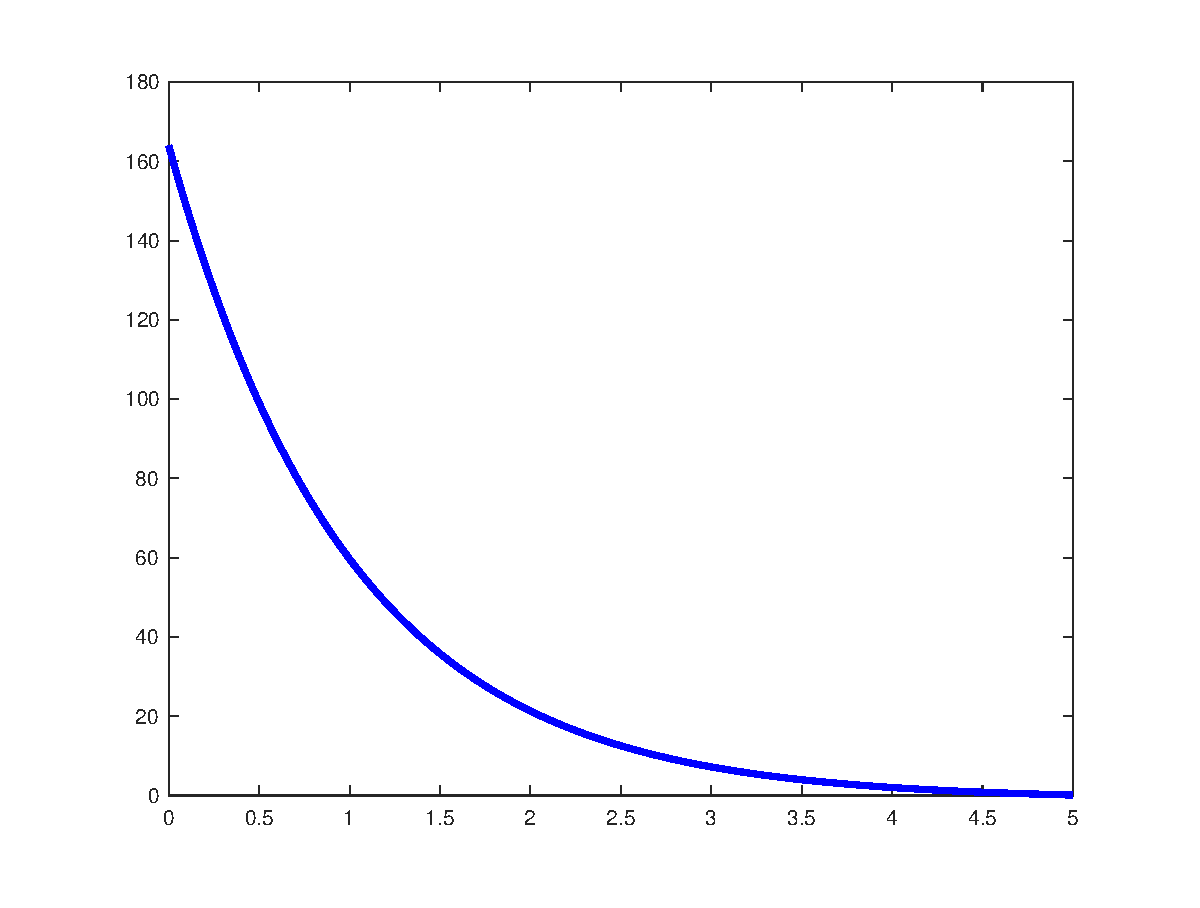
\includegraphics[width=1.5\imagewidth]{Model2-optc.eps}
    \caption{Optimal Control - Model 2}
    \label{fig:model2_optc}
\end{figure}


\begin{figure}[!ht]
    \centering
    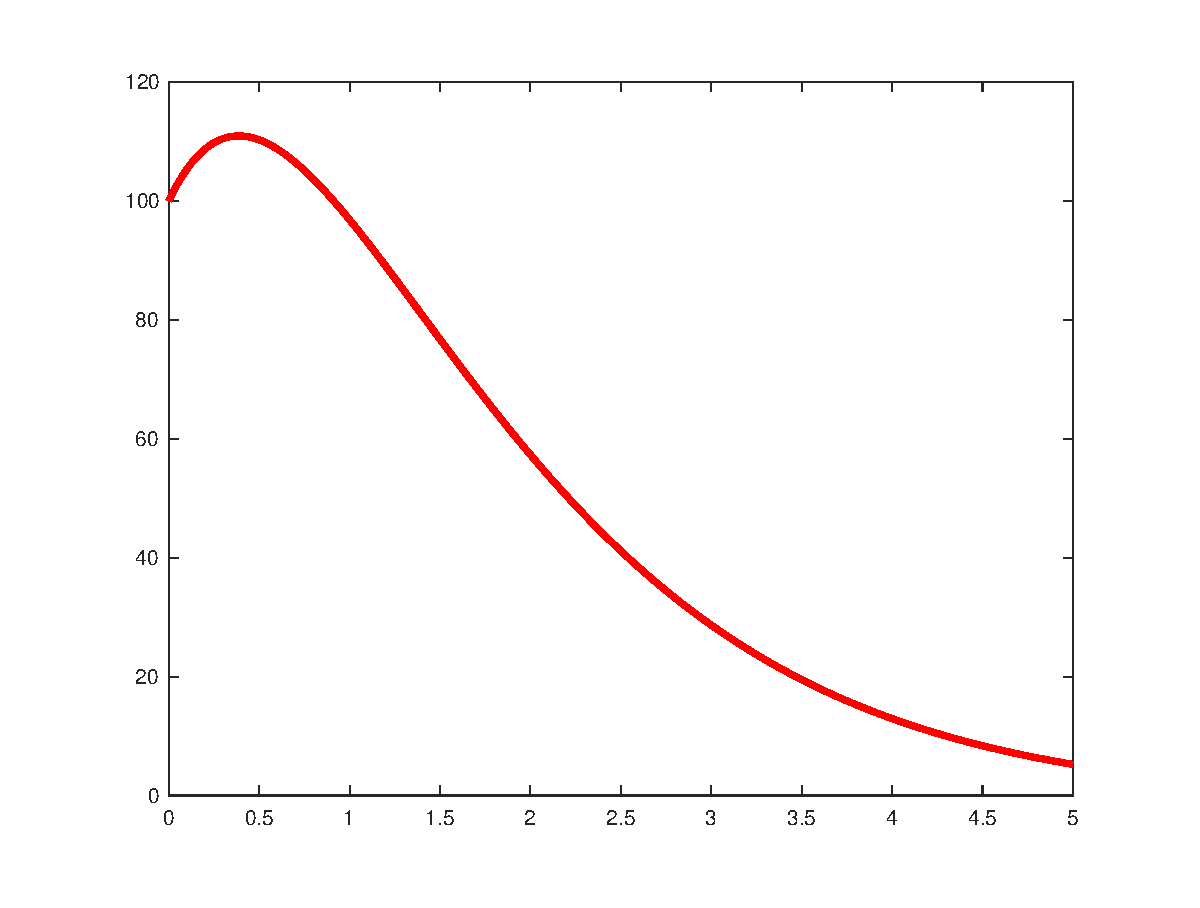
\includegraphics[width=1.5\imagewidth]{Model2-optt.eps}
    \caption{Total Pollution - Model 2}
    \label{fig:model2_optt}
\end{figure}
